% !TeX program = xelatex
\documentclass[aspectratio=169]{beamer}

% --- Math ---
\usepackage{amsmath,amssymb,amsfonts,mathtools}

% --- Boxes / Tables ---
\usepackage{booktabs}
\usepackage{tcolorbox}
\usepackage{xcolor}

% --- Persian (load late) ---
\usepackage{xepersian}
\settextfont{XB Niloofar} % فونت را مطابق سیستم خودت عوض کن
\setlatintextfont{Times New Roman}
\setdigitfont{XB Niloofar}

% --- Beamer theme ---
\usetheme{Madrid}
\usecolortheme{default}
\setbeamertemplate{navigation symbols}{}

% --- Hyperref setup (beamer loads it) ---
\hypersetup{
  unicode=true,
  pdfencoding=auto
}

% --- Commands ---
\newcommand{\E}{\mathbb{E}}
\newcommand{\cX}{\mathcal{X}}
\newcommand{\eps}{\varepsilon}

% --- Title ---
\title[بندیت پیوسته لیپ‌شیتز]{تلاش‌هایی برای پیدا کردن کران بالایی بهتر\\ برای مسئله بندیت پیوسته و لیپ‌شیتز}
\author{حامی‌ عبادزاده \and مهدی دارابی}
\institute{درس: آنالیز احتمالات ابعاد بالا \\ دانشگاه صنعتی شریف}
\date{۲ اسفند ۱۴۰۴}

\begin{document}

\begin{frame}
  \titlepage
\end{frame}

\begin{frame}
\centering
\vfill
{\Large به نام خدا}
\vfill
\end{frame}

\begin{frame}{فهرست مطالب}
  \tableofcontents
\end{frame}

% =========================================================
\section{مقدمه و شهود مسئله}

\begin{frame}{مقدمه: موازنه اکتشاف/بهره‌برداری}
\begin{LTR}
\begin{columns}[T,onlytextwidth]
  \begin{column}{0.45\textwidth}
    \centering
    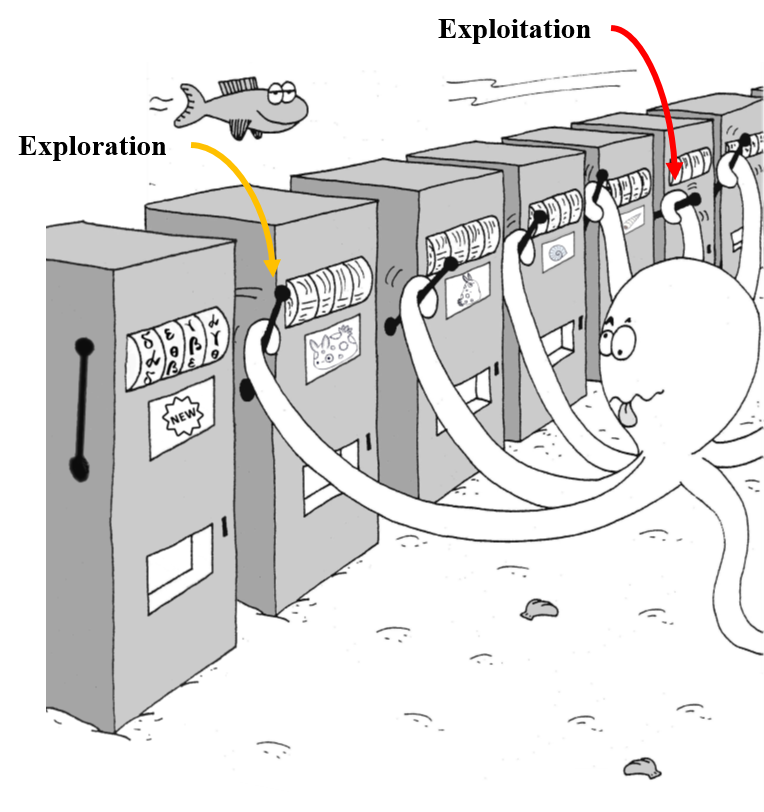
\includegraphics[width=\linewidth]{figs/octopus.png}
  \end{column}
  \begin{column}{0.55\textwidth}
    \begin{RTL}
    \raggedright
    \begin{itemize}
      \item در تصمیم‌گیری تکرارشونده، کیفیت واقعی گزینه‌ها از پیش معلوم نیست.
      \item باید هم‌زمان:
      \begin{itemize}
        \item \textbf{اکتشاف}: آزمون گزینه‌های کمترشناخته برای کسب اطلاعات،
        \item \textbf{بهره‌برداری}: استفاده از گزینه‌هایی که تاکنون بهتر بوده‌اند.
      \end{itemize}
      \item هدف: کمینه‌کردن \textbf{پشیمانی} در افق زمانی.
    \end{itemize}
    \end{RTL}
  \end{column}
\end{columns}
\end{LTR}
\end{frame}

% =========================================================
\section{تعریف رسمی: بندیت گسسته}

\begin{frame}{تعریف: بندیت چندبازویی}
\begin{itemize}
  \item $K$ بازو؛ برای هر بازو $i$ دنباله پاداش‌ها $Y_{i,1},Y_{i,2},\dots$ مستقل و هم‌توزیع با توزیع ناشناخته $P_i$.
  \item $\mu_i:=\E[Y_{i,1}]$ و فرض می‌کنیم پاداش‌ها در بازه $[0,1]$ کراندارند.
  \item $T_i(n)$ تعداد دفعات انتخاب بازوی $i$ تا پایان گام $n$.
\end{itemize}
\[
\E\!\left[\sum_{i=1}^K \sum_{s=1}^{T_i(n)} Y_{i,s}\right]
= \sum_{i=1}^K \mu_i \, \E[T_i(n)].
\]
\end{frame}

\begin{frame}{پشیمانی (Regret)}
\[
\mu^\star:=\max_{1\le i\le K}\mu_i,
\qquad
R(n):=\mu^\star n-\sum_{i=1}^K \mu_i\,\E[T_i(n)].
\]
هدف: طراحی سیاستی با $R(n)$ کوچک.
\end{frame}

% =========================================================
\section{UCB1}

\begin{frame}{UCB1: شاخص}
\[
\widehat{\mu}_i(t-1)=\frac{1}{T_i(t-1)}\sum_{s=1}^{T_i(t-1)}Y_{i,s},
\qquad
I_i(t)=\widehat{\mu}_i(t-1)+\sqrt{\frac{2\ln n}{T_i(t-1)}}.
\]
\begin{itemize}
  \item جمله اول: بهره‌برداری.
  \item جمله دوم: اکتشاف (عدم‌قطعیت).
\end{itemize}
\end{frame}

\begin{frame}{الگوریتم \lr{UCB1}}
\begin{tcolorbox}[colback=white, title=UCB1]
\begin{enumerate}
\item \textbf{مقداردهی اولیه:} هر بازو $i=1,\dots,K$ را دقیقاً یک‌بار انتخاب کن و پاداش را ثبت کنید.
\item \textbf{برای هر گام} $t=K+1,\dots,T$:
\begin{itemize}
  \item برای هر بازو $i$ شاخص زیر را محاسبه کنید:
  \[
  I_i(t)=\widehat{\mu}_i(t-1)+\sqrt{\frac{2\ln n}{T_i(t-1)}}.
  \]
  \item بازوی با بیشترین شاخص را انتخاب کنید و پاداش را ثبت کنید.
\end{itemize}
\end{enumerate}
\end{tcolorbox}
\end{frame}


\begin{frame}{\lr{UCB1}: کران پشیمانیِ وابسته به شکاف}
\[
\Delta_i := \mu^\star-\mu_i \quad (\text{برای بازوهای زیرِبهینه})
\]

\begin{tcolorbox}[colback=white, title=نتیجه کلاسیک]
\[
\E[T_i(n)] \le \frac{8\ln n}{\Delta_i^2}+1+\frac{\pi^2}{3}
\]
\vspace{-6pt}
\[
R(n)\le \sum_{i:\Delta_i>0}\left(\frac{8\ln n}{\Delta_i}+\Bigl(1+\frac{\pi^2}{3}\Bigr)\Delta_i\right)
\]
\end{tcolorbox}
\end{frame}

% =========================================================
\section{بندیت پیوسته و فرض لیپ‌شیتز}

\begin{frame}{تعریف: بندیت پیوسته}
\begin{itemize}
  \item فضای عمل: $\cX$ (مثلاً زیرمجموعه‌ای فشرده از $\mathbb{R}^d$).
  \item در گام $t$ عمل $X_t\in\cX$ و پاداش $Y_t\in[0,1]$.
  \item تابع میانگین: $f(x)=\E[Y_t\mid X_t=x]$ و $f^\star=\sup_{x\in\cX}f(x)$.
\end{itemize}
\[
R(n)=\sum_{t=1}^n \E\bigl[f^\star-f(X_t)\bigr].
\]
\end{frame}

\begin{frame}{فرض لیپ‌شیتز}
اگر برای ثابت $L>0$ داشته باشیم
\[
|f(x)-f(x')|\le L\,d(x,x')\qquad(\forall x,x'\in\cX),
\]
آن‌گاه اعمال نزدیک، میانگین پاداش نزدیک دارند و «ساختار هندسی» قابل استفاده می‌شود.
\end{frame}


\begin{frame}{شهود لیپ‌شیتز}
  \vspace{-8pt}
\begin{figure}
  \centering
  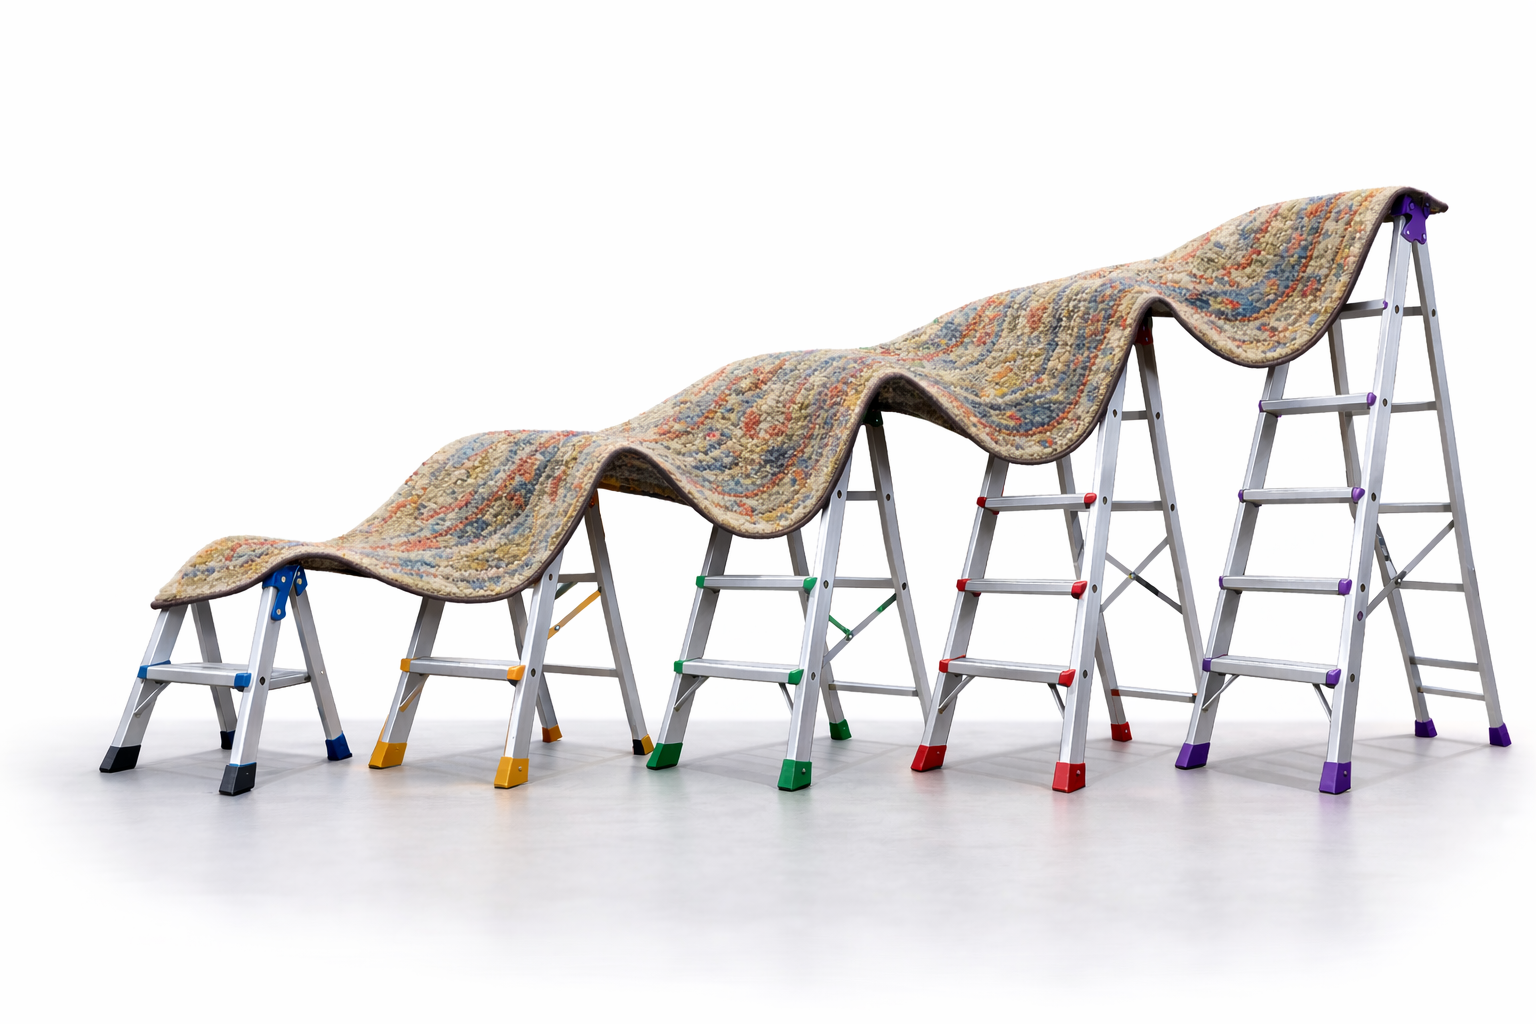
\includegraphics[width=0.70\linewidth]{figs/ladders_carpet.png}
\end{figure}

\vspace{-50pt}
\begin{block}{پیام شهودی}
اگر ورودی‌ها (نقاط) نزدیک باشند، خروجی‌ها نمی‌توانند «پرش» بزرگی داشته باشند؛
شیب تغییرات با یک ثابت $L$ کنترل می‌شود.
\end{block}
\end{frame}


\begin{frame}{مثال قیمت‌گذاری و توجیه فرض لیپ‌شیتز}
\vspace{-8pt}
  \begin{block}{سناریو (کنش = قیمت)}
فرض کنید کنش شما انتخاب یک قیمت باشد:
\[
x\in[0,1].
\]
در هر مرحله، قیمت $x$ را اعلام می‌کنید و درآمد تصادفی زیر را مشاهده می‌کنید:
\[
Y = x\cdot \mathbf{1}\{\text{مشتری با قیمت \lr{x} خرید می‌کند}\}.
\]
\end{block}

\vspace{-7pt}
\begin{block}{تابع میانگین پاداش}
تابع پاداش میانگین (میانگین شرطی درآمد) برابر است با:
\[
f(x)=\E[Y\mid X=x]=x\,p(x),
\]
که در آن $p(x)$ احتمال خرید در قیمت $x$ است.
\end{block}

\vspace{-6pt}
در بسیاری از بازارها، تغییرات کوچک در قیمت معمولاً باعث «جهش ناگهانی» در $p(x)$ نمی‌شود؛
پس $p(x)$ و در نتیجه $f(x)$ به‌طور تدریجی تغییر می‌کنند.
این دقیقاً همان شهودی است که فرض لیپ‌شیتز برای $f$ بیان می‌کند.
\end{frame}

% =========================================================
\section{گسسته‌سازی با $\eps$-پوشش و سیاست پیشنهادی}

\begin{frame}{گسسته‌سازی با $\eps$-پوشش}
اگر $(\cX,d)$ فضای متریک باشد، $N_\eps\subset\cX$ یک $\eps$-پوشش است اگر:
\[
\forall x\in\cX\ \exists \tilde{x}\in N_\eps:\ d(x,\tilde{x})\le \eps
\]
اگر
\[
N_\eps=\{x_1,\dots,x_K\},\qquad K:=|N_\eps|
\]
می‌توان نقاط شبکه را به عنوان بازوهای یک مسئله گسسته در نظر گرفت و UCB1 را روی آن اجرا کرد.
\end{frame}

\begin{frame}{مسئله پیشنهادی}
\begin{block}{پرسش اصلی}
اگر در مسئله‌ی بندیتِ پیوسته با پاداش‌های کراندار، تابع میانگین پاداش $f$ لیپ‌شیتز باشد،
آیا می‌توان با گسسته‌سازی فضای عمل از طریق یک $\eps$-پوشش و اجرای مستقیم الگوریتم \lr{UCB1}
روی مجموعه‌ی گسسته‌ی $N_\eps$، به کران پشیمانی‌ای دست یافت که (با انتخاب مناسب $\eps$)
از کران ارائه‌شده در حالت پیوسته \;(\text{قضیه ۱})\; بهتر باشد؟
\end{block}

\vspace{6pt}
\begin{itemize}
\item فضای عمل: $\mathcal{X}$، تابع میانگین: $f:\mathcal{X}\to[0,1]$.
\item $N_\eps\subset\mathcal{X}$ یک $\eps$-پوشش و $|N_\eps|<\infty$.
\item سیاست پیشنهادی: محدود کردن انتخاب‌ها به $N_\eps$ و اجرای \lr{UCB1} روی آن.
\end{itemize}
\end{frame}


\begin{frame}[plain]
\centering
\vfill
{\Huge \bfseries تلاش‌ها}
\vfill
\end{frame}


\begin{frame}{تلاش اول: گسسته‌سازی با $\eps$-پوشش و اجرای \lr{UCB1}}
\begin{itemize}
  \item \textbf{ایده:} فضای پیوسته‌ی عمل $\mathcal{X}$ را با یک $\eps$-پوشش $N_\eps$ تقریب می‌زنیم
  و انتخاب‌ها را به $N_\eps$ محدود می‌کنیم.
  \item سپس مسئله به یک بندیت \textbf{گسسته} با $K:=|N_\eps|$ بازو تبدیل می‌شود
  و \lr{UCB1} را روی این $K$ بازو اجرا می‌کنیم.
  \item پشیمانی کل به دو مؤلفه تفکیک می‌شود:
  \[
  \text{(خطای گسسته‌سازی)}\;+\;\text{(پشیمانی روی شبکه)}.
  \]
  \item در ادامه، $\eps$ را طوری انتخاب می‌کنیم که این دو مؤلفه متعادل شوند.
\end{itemize}
\end{frame}


\begin{frame}{سیاست «گسسته‌سازی + UCB1»}
\begin{tcolorbox}[title=ایده اصلی]
فقط از مجموعه محدود $N_\eps$ عمل انتخاب کنید:
\[
X_t\in N_\eps
\]
و UCB1 را روی بازوهای متناظر با $\{x_1,\dots,x_K\}$ اجرا کن، با میانگین بازوی $i$ برابر:
\[
\mu_i=f(x_i)
\]
\end{tcolorbox}

پشیمانی نسبت به بهینۀ پیوسته:
\[
R(n)=\sum_{t=1}^n \bigl(\E[f^\star-f(X_t)]\bigr)
\]
\end{frame}







% =========================================================
\section{تلاش اول: کران بالا با گسسته‌سازی}

\begin{frame}{لم ۱: خطای تقریب شبکه (کنترل با لیپ‌شیتز)}
\begin{block}{بیان لم و اثبات کوتاه}
فرض کنید $N_\eps$ یک $\eps$-پوشش از $\chi$ و $f$ با ثابت $L$ لیپ‌شیتز باشد. تعریف کنید
\[
f^\star:=\sup_{x\in\chi} f(x),\qquad f^\star_\eps:=\max_{x\in N_\eps} f(x).
\]
آنگاه
\[
0\le f^\star-f^\star_\eps \le L\eps.
\]

{\footnotesize
\textbf{اثبات کوتاه.}
بگذارید $x^\star\in\arg\max_{x\in\chi} f(x)$.
چون $N_\eps$ یک $\eps$-پوشش است، نگاشتی $\pi:\chi\to N_\eps$ وجود دارد به‌طوری‌که
\[
d\bigl(x,\pi(x)\bigr)\le \eps\qquad(\forall x\in\chi).
\]
در نتیجه
\[
f^\star=f(x^\star)\le f\bigl(\pi(x^\star)\bigr)+L\eps \le f^\star_\eps+L\eps.
\]
پس $f^\star-f^\star_\eps\le L\eps$ و از طرفی بدیهی است $f^\star_\eps\le f^\star$.}
\end{block}
\end{frame}


\begin{frame}{نتیجه‌ی لم ۱: تجزیه و کران پشیمانی}
اگر $X_t\in N_\eps$ (یعنی سیاست فقط از نقاط شبکه انتخاب کند)، آنگاه
\[
R(n):=\sum_{t=1}^n\bigl(\E[f^\star-f(X_t)]\bigr)
=
\sum_{t=1}^n\bigl(\E[f^\star-f^\star_\eps]\bigr)
+
\sum_{t=1}^n\bigl(\E[f^\star_\eps-f(X_t)]\bigr)
\le
L\eps n + R_n^\eps,
\]
که در آن
\[
R_n^\eps:=\sum_{t=1}^n\bigl(\E[f^\star_\eps-f(X_t)]\bigr)
\]
پشیمانی نسبت به بهترین نقطه روی شبکه است.
\end{frame}


\begin{frame}{لم ۲: کران مستقل از فاصله برای UCB1 روی $K$ بازو}
در مسئله گسسته با $K$ بازو و پاداش‌های $[0,1]$، پشیمانی مورد انتظار UCB1 پس از $T$ گام:
\[
R_n^\eps\le 4\sqrt{2K \times n\ln (n)}+\Bigl(1+\frac{\pi^2}{3}\Bigr)K
\]
\begin{itemize}
  \item ایده اثبات: بازوها را با آستانه $\alpha$ به «نزدیک‌بهینه» و «دور از بهینه» تقسیم می‌کنیم.
  \item برای نزدیک‌بهینه‌ها: $\le \alpha n$.
  \item برای دورها: از کران کلاسیک $\E[T_i(n)]$ استفاده می‌کنیم.
  \item انتخاب بهینه $\alpha=\sqrt{(8K\ln (n))/n}$ دو جمله اصلی را هم‌مرتبه می‌کند.
\end{itemize}
\end{frame}

\begin{frame}{ترکیب لم‌ها: کران نهاییِ تلاش اول}
از لم ۱ و لم ۲:
\[
R(n)\le L\eps n + 4\sqrt{2K \times n\ln (n)}+\Bigl(1+\frac{\pi^2}{3}\Bigr)K
\]
برای $\cX=[0,1]^d$ با متریک $\|\cdot\|_\infty$ می‌توان پوششی با
\[
K=|N_\eps|\ \lesssim\ \left(\frac{1}{\eps}+1\right)^d \approx \eps^{-d}
\]
در نظر گرفت.

با انتخاب
\[
\eps:=n^{-1/(d+2)}\quad\Rightarrow\quad K=\eps^{-d}=n^{d/(d+2)}
\]
به دست می‌آید:
\begin{tcolorbox}[colback=yellow, colframe=blue!70!black, boxrule=0.8pt,
                  left=6pt,right=6pt,top=6pt,bottom=6pt]
\[
R(n) \le\ L\,n^{\frac{d+1}{d+2}}
\;+\;4\sqrt{2\ln (n)}\,n^{\frac{d+1}{d+2}}
\;+\;\Bigl(1+\frac{\pi^2}{3}\Bigr)n^{\frac{d}{d+2}} .
\]
\end{tcolorbox}
\end{frame}

\begin{frame}{جمع‌بندی تلاش اول}
\begin{itemize}
  \item سیاست ساده: شبکه‌سازی $\eps$ و اجرای مستقیم UCB1 روی شبکه.
  \item دو منبع پشیمانی:
  \begin{itemize}
    \item خطای گسسته‌سازی: $L\eps n$
    \item پشیمانی گسسته UCB1 روی $K$ بازو
  \end{itemize}
  \item بهینه‌سازی $\eps$ نرخ اصلی را از جنس $n^{\frac{d+1}{d+2}}$ (با عامل $\sqrt{\ln (n)}$) می‌دهد.
\end{itemize}
\end{frame}





% =========================================================
\section{تلاش دوم: ایده ناموفقِ کران با سوپریمم یک فرایند}
\begin{frame}{تلاش دوم (ناموفق): بازنویسی پشیمانی به‌صورت کران از بالا برای امید سوپریمم یک فرایند}

\begin{block}{انگیزه}
ایده‌ی این تلاش استفاده از لم زیر بود که «امید سوپریمم» یک فرایند تصادفیِ لیپ‌شیتز و زیرگاوسی را
با عدد پوشش کنترل می‌کند. به‌طور خلاصه، اگر $\{Z_t\}_{t\in T}$ یک فرایند لیپ‌شیتز و زیرگاوسی باشد، آنگاه کرانی از شکل زیر برقرار است:
\[
\E\!\left[\sup_{t\in T} Z_t\right]
\ \le\ 
\eps\,\E[C]
\;+\;
\sqrt{2\sigma^2\log N(T,d,\eps)}.
\]
\end{block}

\smallskip
در این‌جا $C$ ثابت لیپ‌شیتز، $\sigma^2$ پارامتر زیرگاوسی است.
\end{frame}

\begin{frame}{انگیزه تلاش دوم: لم سوپریمم فرایند زیرگاوسی}
هدف: بازنویسی پشیمانی به شکل
\[
R(n)\le \E\Big[\sup_{x\in\cX} Z_x\Big]
\]
به گونه‌ای که فرایند $\{Z_x\}_{x\in\cX}$:
\begin{itemize}
  \item نسبت به $x$ \textbf{لیپ‌شیتز} باشد،
  \item \textbf{زیرگاوسیِ مرکزدار} باشد،
\end{itemize}
تا بتوان امید سوپریمم را با \emph{عدد پوشش} کنترل کرد.
\end{frame}

\begin{frame}{یک انتخاب وسوسه‌انگیز و مشکل بنیادی}
انتخاب صوری:
\[
Z_x := n \times f(x) - \sum_{t=1}^n f(X_t)
\]
\begin{itemize}
  \item اگر $x^\star\in\arg\max f(x)$، آنگاه $Z_{x^\star}$ «شبیه» پشیمانیِ مبتنی بر $f$ است.
  \item اگر $f$ لیپ‌شیتز باشد:
  \[
  |Z_x-Z_{x'}|=n \times |f(x)-f(x')|\le n \times L\,d(x,x')
  \]
  پس فرایند نسبت به $x$ لیپ‌شیتز است.
  \item چون $f(\cdot)\in[0,1]$، داریم $-n\le Z_x\le n$ و در نتیجه کران‌دار/زیرگاوسی است.
\end{itemize}

\textbf{مشکل اصلی:} $Z_x$ \textbf{مرکزی نیست}:
\[
\E[Z_x]=n \times f(x)-\sum_{t=1}^n \E[f(X_t)]\neq 0
\]
\end{frame}

\begin{frame}{مرکزی‌سازی و از بین رفتن وابستگی به $x$}
اگر مرکزی کنیم:
\[
\widetilde{Z}_x:=Z_x-\E[Z_x]
\]
آنگاه:
\[
\widetilde{Z}_x
=
\Bigl(n \times f(x)-\sum_{t=1}^n f(X_t)\Bigr)
-
\Bigl(n \times f(x)-\sum_{t=1}^n \E[f(X_t)]\Bigr)
=
-\sum_{t=1}^n f(X_t)+\sum_{t=1}^n \E[f(X_t)]
\]
که دیگر \textbf{به $x$ وابسته نیست}. پس:
\[
\sup_{x\in\cX}\widetilde{Z}_x=\widetilde{Z}_x,\qquad
\E\Big[\sup_{x\in\cX}\widetilde{Z}_x\Big]=\E[\widetilde{Z}_x]=0
\]
بنابراین این مسیر در بهترین حالت «کران صفر» برای کمیت مرکزی می‌دهد و عملاً کران مفیدی برای پشیمانی تولید نمی‌کند.
\end{frame}

\begin{frame}{کران بدیهی پشیمانی (بدون ساختار بیشتر)}
چون در هر گام:
\[
0\le f^\star-f(X_t)\le 1
\]
داریم:
\[
0\le R(n)=\sum_{t=1}^n \E[f^\star-f(X_t)]\le n
\quad\Rightarrow\quad
R(T) \le n
\]
و تلاش دوم در نهایت به چیزی بهتر از این نرخ عمومی نرسید.
\end{frame}

% =========================================================
\section{نتیجه‌گیری و مسیرهای ادامه}


\begin{frame}{جمع‌بندیِ تلاش دوم (ناموفق)}
\begin{itemize}
  \item هدف: کران‌گذاری پشیمانی با بازنویسی آن به شکل $\E[\sup_{x\in\mathcal{X}} Z_x]$ و استفاده از لم سوپریممِ فرایند لیپ‌شیتز–زیرگاوسی.
  \item مانع: نتوانستیم فرایندی بسازیم که هم وابستگی به $x$ را حفظ کند و هم مرکزدار/زیرگاوسی باشد.
  \item نتیجه: بهترین کرانِ حاصل هم‌مرتبه با کران بدیهی $R(n)\le n$ (یعنی $O(n)$) شد.
\end{itemize}
\end{frame}

\begin{frame}{نتیجه‌گیری}
\begin{itemize}
  \item \textbf{تلاش اول (موفق)}: گسسته‌سازی با $\eps$-پوشش + UCB1
  \[
  R(n)\ \lesssim\ n^{\frac{d+1}{d+2}}\sqrt{\ln (n)}\ \ (+\ \text{جملات پایین‌تر})
  \]
  \item \textbf{تلاش دوم (ناموفق)}: ساخت فرایند $Z_x$ برای کنترل $\E[\sup_x Z_x]$
  \begin{itemize}
    \item چالشِ مرکزدار بودن و حفظ وابستگی به $x$
    \item مرکزی‌سازی وابستگی به $x$ را از بین برد
  \end{itemize}
\end{itemize}
\end{frame}

\begin{frame}{مراجع}
\begin{thebibliography}{9}
\bibitem{auer2002}
Peter Auer, Nicol\`o Cesa-Bianchi, and Paul Fischer.
\newblock Finite-time analysis of the multiarmed bandit problem.
\newblock \emph{Machine Learning}, 47(2--3):235--256, 2002.
\end{thebibliography}
\end{frame}

\end{document}